\section{Shortest Path of DAGs and Shortest Path Tree}

\subsection*{Shortest Path of DAGs}
Let $G = (V, E)$ be a DAG with possibly negative edge length $c(e)$ for each $e\in E$.
We want to find the distance from a given source $s$ to each vertex $v\in V$.
Note that $G$ does not contain negative cycles simply because $G$ does not contain any cycle.
We can design a simpler version of Bellman-Ford algorithm to solve this problem.
In particular, we only need to do one round of ``update''~(instead of $|V|-1$ rounds as in Bellman-Ford algorithm).
But, the edges cannot be updated in a arbitrary order. In fact,
we first need to find a linearization of $G$~(recall that a directed graph can be linearized if and only if it's a DAG),
and then update the in-edges of vertices following this linearization.

%%\begin{minipage}{0.8\textwidth}
%%	\aaA {5}{procedure update~(edge $(u,v)\in E$)}\xxx
%%	\aaB {3}{if~($dist[v] > dist[u] + l(u,v)$)}\xxx
%%	\aac {$dist[v] = dist[u] + l(u,v)$;}\xxx
%%	\aac {\textcolor{black}{$prev[v]= u$};}\xxx
%%	\aab {end if;}\xxx
%%	\aaa {end procedure;}\xxx
%%\end{minipage}

\begin{minipage}{0.8\textwidth}
	\aaA {10}{Algorithm DP-shortest-path~(DAG $G = (V, E)$, $l(e)$ for any $e\in E$, $s \in V$)}\xxx
	\aab {init array $dist$ of size $|V|$: $dist[s] = 0$; $dist[v] = \infty$ for any $v\neq s$;}\xxx
	\aab {calculate a linearization of $G$;}\xxx
	\aaB {4}{\textcolor{blue}{for $v\in V$ following the order of linearization}}\xxx
	\aaC {2}{for each $(u,v)\in E$;}\xxx
	\aad {$update(u,v)$;}\xxx
	\aac {end for;}\xxx
	\aab {end for;}\xxx
	\aab {for each $v\in V$: report: $distance(s,v) = dist[v]$;}\xxx
	\aaa {end algorithm;}\xxx
\end{minipage}


The correctness of above algorithm for DAGs can also be proved in the same way as in the Bellman-Ford algorithm.
Let $p = s \to a \to b \to \cdots \to u \to v$ be the shortest path from $s$ to $v$;
we have proved that~(for Bellman-Ford algorithm), if the run of the algorithm contains a \emph{subsequence} of update procedures
that sequentially update the edges in the shortest path, then 
$dist[v]$ will be equal to $distance(s,v)$ after these update procedures.
Our above algorithm update the in-edges of vertices sequentially following a linearization.
In a DAG, the list of vertices of any path, including shortest path, must be a \emph{subsequence}
of the linearization. Therefore, the list of edges of any path must be updated
sequentially by the algorithm. See Figure~\ref{fig:dag}.

\begin{figure}[h]
\centering{

\tikzset{every picture/.style={line width=0.75pt}} %set default line width to 0.75pt        

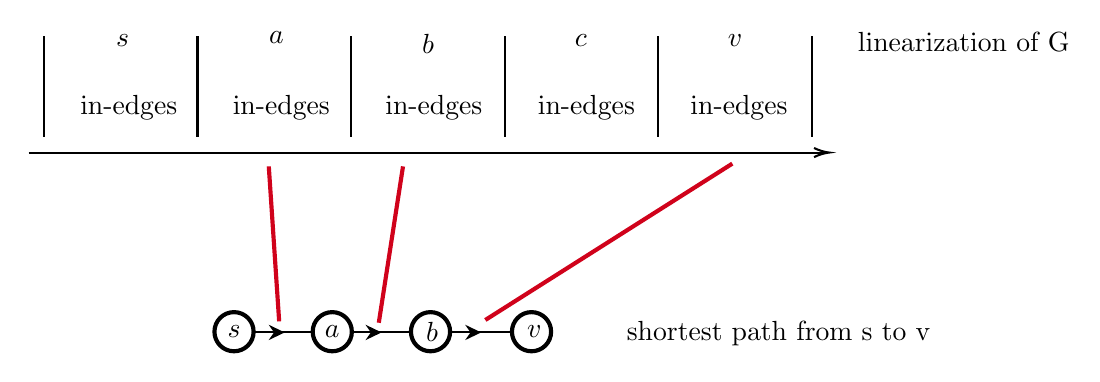
\begin{tikzpicture}[x=0.5pt,y=0.5pt,yscale=-1,xscale=1]
%uncomment if require: \path (0,286); %set diagram left start at 0, and has height of 286

%Straight Lines [id:da42563372855460047] 
\draw [color={rgb, 255:red, 0; green, 0; blue, 0 }  ,draw opacity=1 ][line width=0.75]    (250.5,248) -- (293.5,248) ;
\draw [shift={(272,248)}, rotate = 180] [fill={rgb, 255:red, 0; green, 0; blue, 0 }  ,fill opacity=1 ][line width=0.08]  [draw opacity=0] (11.61,-5.58) -- (0,0) -- (11.61,5.58) -- (7.71,0) -- cycle    ;
%Straight Lines [id:da13574797376852343] 
\draw [color={rgb, 255:red, 0; green, 0; blue, 0 }  ,draw opacity=1 ][line width=0.75]    (322.5,248) -- (365.5,248) ;
\draw [shift={(344,248)}, rotate = 180] [fill={rgb, 255:red, 0; green, 0; blue, 0 }  ,fill opacity=1 ][line width=0.08]  [draw opacity=0] (11.61,-5.58) -- (0,0) -- (11.61,5.58) -- (7.71,0) -- cycle    ;
%Straight Lines [id:da9930965641121888] 
\draw    (17,118) -- (593.5,118) ;
\draw [shift={(595.5,118)}, rotate = 180] [color={rgb, 255:red, 0; green, 0; blue, 0 }  ][line width=0.75]    (10.93,-3.29) .. controls (6.95,-1.4) and (3.31,-0.3) .. (0,0) .. controls (3.31,0.3) and (6.95,1.4) .. (10.93,3.29)   ;
%Straight Lines [id:da09874107164515367] 
\draw [color={rgb, 255:red, 0; green, 0; blue, 0 }  ,draw opacity=1 ][line width=0.75]    (180.5,248) -- (223.5,248) ;
\draw [shift={(202,248)}, rotate = 180] [fill={rgb, 255:red, 0; green, 0; blue, 0 }  ,fill opacity=1 ][line width=0.08]  [draw opacity=0] (11.61,-5.58) -- (0,0) -- (11.61,5.58) -- (7.71,0) -- cycle    ;
%Straight Lines [id:da6519777460675502] 
\draw [color={rgb, 255:red, 208; green, 2; blue, 27 }  ,draw opacity=1 ][line width=1.5]    (198,240) -- (190.5,128) ;
%Straight Lines [id:da29298485524387174] 
\draw [color={rgb, 255:red, 208; green, 2; blue, 27 }  ,draw opacity=1 ][line width=1.5]    (270,241) -- (287.5,128) ;
%Straight Lines [id:da3208602618624562] 
\draw [color={rgb, 255:red, 208; green, 2; blue, 27 }  ,draw opacity=1 ][line width=1.5]    (347,239) -- (525.5,126) ;
%Straight Lines [id:da3600584205418621] 
\draw    (139,34) -- (139,107) ;
%Straight Lines [id:da02657749763727446] 
\draw    (250,34) -- (250,107) ;
%Straight Lines [id:da432596125208347] 
\draw    (361,34) -- (361,107) ;
%Straight Lines [id:da23108993646686993] 
\draw    (472,34) -- (472,107) ;
%Straight Lines [id:da4614439049417304] 
\draw    (583,34) -- (583,107) ;
%Straight Lines [id:da16560659557639468] 
\draw    (28,34) -- (28,107) ;

% Text Node
\draw  [line width=1.5]   (165.38, 247.47) circle [x radius= 14.15, y radius= 14.15]   ;
\draw (165.38,247.47) node   [align=left] {$\displaystyle s$};
% Text Node
\draw  [line width=1.5]   (236.38, 247.47) circle [x radius= 14.15, y radius= 14.15]   ;
\draw (236.38,247.47) node   [align=left] {$\displaystyle a$};
% Text Node
\draw  [line width=1.5]   (307.38, 247.47) circle [x radius= 14.15, y radius= 14.15]   ;
\draw (301.88,247.47) node [anchor=west] [inner sep=0.75pt]   [align=left] {$\displaystyle b$};
% Text Node
\draw  [line width=1.5]   (380.38, 247.47) circle [x radius= 14.15, y radius= 14.15]   ;
\draw (374.88,247.47) node [anchor=west] [inner sep=0.75pt]   [align=left] {$\displaystyle v$};
% Text Node
\draw (614,29) node [anchor=north west][inner sep=0.75pt]   [align=left] {linearization of G};
% Text Node
\draw (447,238) node [anchor=north west][inner sep=0.75pt]   [align=left] {shortest path from s to v};
% Text Node
\draw (52,74) node [anchor=north west][inner sep=0.75pt]   [align=left] {in-edges};
% Text Node
\draw (188.5,28.5) node [anchor=north west][inner sep=0.75pt]   [align=left] {$\displaystyle a$};
% Text Node
\draw (299,30.5) node [anchor=north west][inner sep=0.75pt]   [align=left] {$\displaystyle b$};
% Text Node
\draw (409.5,30.5) node [anchor=north west][inner sep=0.75pt]   [align=left] {$\displaystyle c$};
% Text Node
\draw (520,30.5) node [anchor=north west][inner sep=0.75pt]   [align=left] {$\displaystyle v$};
% Text Node
\draw (78,30.5) node [anchor=north west][inner sep=0.75pt]   [align=left] {$\displaystyle s$};
% Text Node
\draw (162.25,74) node [anchor=north west][inner sep=0.75pt]   [align=left] {in-edges};
% Text Node
\draw (272.5,74) node [anchor=north west][inner sep=0.75pt]   [align=left] {in-edges};
% Text Node
\draw (382.75,74) node [anchor=north west][inner sep=0.75pt]   [align=left] {in-edges};
% Text Node
\draw (493,74) node [anchor=north west][inner sep=0.75pt]   [align=left] {in-edges};


\end{tikzpicture}

}
\caption{Illustration of the correctness of the DP algorithm for DAGs.}
\label{fig:dag}
\end{figure}


\subsection*{Shortest Path Tree}

So far we have designed three algorithms, BFS, Dijkstra's algorithm, and Bellman-Ford algorithm
to solve shortest path problems for unit edge length, positive edge length, and possible negative edge length, respectively.
In these algorithm, $dist[v]$ will give the \emph{length} of the
shortest path from $s$ to $v$. How to find the actual shortest path?
Before designing algorithm to find paths~(we will do it by modifying all three algorithm),
let's think about how to store them first.
Recall that we want to store $|V|$ paths, ones from $s$ to each vertex in $V$.
If we implicitly store these $|V|$ paths in a naive way, it may take $O(|V|^2)$ space.
Can we do better?

In fact, we can use linear space to store these $|V|$ shortest paths from a single source $s$.
Let $G = (V, E)$ be a graph with edge length $l(e)$ for any $e \in E$.
Here we allow negative edge length, but not allow \emph{negative cycle}. %~(we will come back to negative cycle later on).
Let $s \in V$ be a source vertex.  Without loss of generality, assume that $s$ can reach all vertices in $V$.
We say $T$ is a \emph{shortest path tree} of $G$ w.r.t.\ source vertex $s$ if:
\vspace*{-\topsep}
\begin{enumerate}
\item $T$ is a rooted tree and its root is $s$;
\item vertices of $T$ is $V$;
\item edges of $T$ is a subset of $E$;
\item for every $v\in V$, the unique path from $s$ to $v$ in $T$ is one shortest path from $s$ to $v$ in $G$.
\end{enumerate}

A shortest path tree always exists. (Think how to prove it.) 
The underlying reason is the optimal substructure property.
Such tree may not be unique though~(see Figure~\ref{fig:tree}).
As in the shortest path tree, each vertex, except $s$, has exactly one in-edge, we can use an array $prev$ of size $|V|$
to store this tree. Array $prev$ is indexed by the vertices, and for each $v\in V$, $prev[v]$ stores the parent of $v$
in the tree~(see Figure~\ref{fig:tree}).
Such array, which takes linear space, therefore represents the shortest path from $s$ to every vertex.

\begin{figure}[h]
\centering{\tikzset{every picture/.style={line width=0.75pt}} %set default line width to 0.75pt        

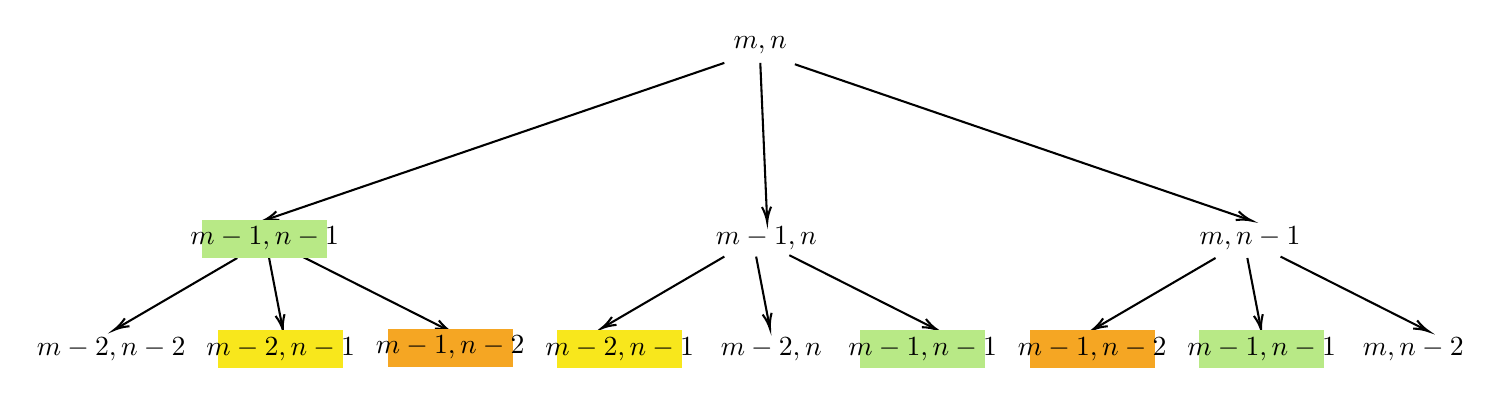
\begin{tikzpicture}[x=0.5pt,y=0.5pt,yscale=-1,xscale=1]
%uncomment if require: \path (0,284); %set diagram left start at 0, and has height of 284

%Straight Lines [id:da1383331413383435] 
\draw    (522.5,36) -- (191.39,149.35) ;
\draw [shift={(189.5,150)}, rotate = 341.1] [color={rgb, 255:red, 0; green, 0; blue, 0 }  ][line width=0.75]    (10.93,-3.29) .. controls (6.95,-1.4) and (3.31,-0.3) .. (0,0) .. controls (3.31,0.3) and (6.95,1.4) .. (10.93,3.29)   ;
%Straight Lines [id:da715204982720897] 
\draw    (548.5,36) -- (553.41,149) ;
\draw [shift={(553.5,151)}, rotate = 267.51] [color={rgb, 255:red, 0; green, 0; blue, 0 }  ][line width=0.75]    (10.93,-3.29) .. controls (6.95,-1.4) and (3.31,-0.3) .. (0,0) .. controls (3.31,0.3) and (6.95,1.4) .. (10.93,3.29)   ;
%Straight Lines [id:da8831806389031782] 
\draw    (573.5,37) -- (901.61,149.35) ;
\draw [shift={(903.5,150)}, rotate = 198.9] [color={rgb, 255:red, 0; green, 0; blue, 0 }  ][line width=0.75]    (10.93,-3.29) .. controls (6.95,-1.4) and (3.31,-0.3) .. (0,0) .. controls (3.31,0.3) and (6.95,1.4) .. (10.93,3.29)   ;
%Straight Lines [id:da6762777724306107] 
\draw    (170.5,177) -- (83.23,227.99) ;
\draw [shift={(81.5,229)}, rotate = 329.7] [color={rgb, 255:red, 0; green, 0; blue, 0 }  ][line width=0.75]    (10.93,-3.29) .. controls (6.95,-1.4) and (3.31,-0.3) .. (0,0) .. controls (3.31,0.3) and (6.95,1.4) .. (10.93,3.29)   ;
%Straight Lines [id:da9537842571445845] 
\draw    (193.5,177) -- (203.12,227.04) ;
\draw [shift={(203.5,229)}, rotate = 259.11] [color={rgb, 255:red, 0; green, 0; blue, 0 }  ][line width=0.75]    (10.93,-3.29) .. controls (6.95,-1.4) and (3.31,-0.3) .. (0,0) .. controls (3.31,0.3) and (6.95,1.4) .. (10.93,3.29)   ;
%Straight Lines [id:da25240177172893863] 
\draw    (217.5,176) -- (322.71,229.1) ;
\draw [shift={(324.5,230)}, rotate = 206.78] [color={rgb, 255:red, 0; green, 0; blue, 0 }  ][line width=0.75]    (10.93,-3.29) .. controls (6.95,-1.4) and (3.31,-0.3) .. (0,0) .. controls (3.31,0.3) and (6.95,1.4) .. (10.93,3.29)   ;
%Straight Lines [id:da4227912867383341] 
\draw    (522.5,176) -- (435.23,226.99) ;
\draw [shift={(433.5,228)}, rotate = 329.7] [color={rgb, 255:red, 0; green, 0; blue, 0 }  ][line width=0.75]    (10.93,-3.29) .. controls (6.95,-1.4) and (3.31,-0.3) .. (0,0) .. controls (3.31,0.3) and (6.95,1.4) .. (10.93,3.29)   ;
%Straight Lines [id:da490335830545392] 
\draw    (545.5,176) -- (555.12,226.04) ;
\draw [shift={(555.5,228)}, rotate = 259.11] [color={rgb, 255:red, 0; green, 0; blue, 0 }  ][line width=0.75]    (10.93,-3.29) .. controls (6.95,-1.4) and (3.31,-0.3) .. (0,0) .. controls (3.31,0.3) and (6.95,1.4) .. (10.93,3.29)   ;
%Straight Lines [id:da44453803269503656] 
\draw    (569.5,175) -- (674.71,228.1) ;
\draw [shift={(676.5,229)}, rotate = 206.78] [color={rgb, 255:red, 0; green, 0; blue, 0 }  ][line width=0.75]    (10.93,-3.29) .. controls (6.95,-1.4) and (3.31,-0.3) .. (0,0) .. controls (3.31,0.3) and (6.95,1.4) .. (10.93,3.29)   ;
%Straight Lines [id:da6159232694423369] 
\draw    (877.5,177) -- (790.23,227.99) ;
\draw [shift={(788.5,229)}, rotate = 329.7] [color={rgb, 255:red, 0; green, 0; blue, 0 }  ][line width=0.75]    (10.93,-3.29) .. controls (6.95,-1.4) and (3.31,-0.3) .. (0,0) .. controls (3.31,0.3) and (6.95,1.4) .. (10.93,3.29)   ;
%Straight Lines [id:da04820263440719896] 
\draw    (900.5,177) -- (910.12,227.04) ;
\draw [shift={(910.5,229)}, rotate = 259.11] [color={rgb, 255:red, 0; green, 0; blue, 0 }  ][line width=0.75]    (10.93,-3.29) .. controls (6.95,-1.4) and (3.31,-0.3) .. (0,0) .. controls (3.31,0.3) and (6.95,1.4) .. (10.93,3.29)   ;
%Straight Lines [id:da4987937509957987] 
\draw    (924.5,176) -- (1029.71,229.1) ;
\draw [shift={(1031.5,230)}, rotate = 206.78] [color={rgb, 255:red, 0; green, 0; blue, 0 }  ][line width=0.75]    (10.93,-3.29) .. controls (6.95,-1.4) and (3.31,-0.3) .. (0,0) .. controls (3.31,0.3) and (6.95,1.4) .. (10.93,3.29)   ;

% Text Node
\draw (548.38,23.47) node   [align=left] {$\displaystyle m,n$};
% Text Node
\draw  [color={rgb, 255:red, 184; green, 233; blue, 134 }  ,draw opacity=1 ][fill={rgb, 255:red, 184; green, 233; blue, 134 }  ,fill opacity=1 ][line width=0.75]   (145.88,149.97) -- (234.88,149.97) -- (234.88,175.97) -- (145.88,175.97) -- cycle  ;
\draw (190.38,162.97) node   [align=left] {$\displaystyle m-1,n-1$};
% Text Node
\draw (552.88,162.97) node   [align=left] {$\displaystyle m-1,n$};
% Text Node
\draw (902.38,162.97) node   [align=left] {$\displaystyle m,n-1$};
% Text Node
\draw (79.38,242.72) node   [align=left] {$\displaystyle m-2,n-2$};
% Text Node
\draw  [color={rgb, 255:red, 248; green, 231; blue, 28 }  ,draw opacity=1 ][fill={rgb, 255:red, 248; green, 231; blue, 28 }  ,fill opacity=1 ][line width=0.75]   (157.38,229.72) -- (246.38,229.72) -- (246.38,255.72) -- (157.38,255.72) -- cycle  ;
\draw (201.88,242.72) node   [align=left] {$\displaystyle m-2,n-1$};
% Text Node
\draw  [color={rgb, 255:red, 245; green, 166; blue, 35 }  ,draw opacity=1 ][fill={rgb, 255:red, 245; green, 166; blue, 35 }  ,fill opacity=1 ][line width=0.75]   (279.88,228.72) -- (368.88,228.72) -- (368.88,254.72) -- (279.88,254.72) -- cycle  ;
\draw (324.38,241.72) node   [align=left] {$\displaystyle m-1,n-2$};
% Text Node
\draw  [color={rgb, 255:red, 248; green, 231; blue, 28 }  ,draw opacity=1 ][fill={rgb, 255:red, 248; green, 231; blue, 28 }  ,fill opacity=1 ][line width=0.75]   (402.38,229.72) -- (491.38,229.72) -- (491.38,255.72) -- (402.38,255.72) -- cycle  ;
\draw (446.88,242.72) node   [align=left] {$\displaystyle m-2,n-1$};
% Text Node
\draw (556.38,242.72) node   [align=left] {$\displaystyle m-2,n$};
% Text Node
\draw  [color={rgb, 255:red, 184; green, 233; blue, 134 }  ,draw opacity=1 ][fill={rgb, 255:red, 184; green, 233; blue, 134 }  ,fill opacity=1 ][line width=0.75]   (621.38,229.72) -- (710.38,229.72) -- (710.38,255.72) -- (621.38,255.72) -- cycle  ;
\draw (665.88,242.72) node   [align=left] {$\displaystyle m-1,n-1$};
% Text Node
\draw  [color={rgb, 255:red, 245; green, 166; blue, 35 }  ,draw opacity=1 ][fill={rgb, 255:red, 245; green, 166; blue, 35 }  ,fill opacity=1 ][line width=0.75]   (743.88,229.72) -- (832.88,229.72) -- (832.88,255.72) -- (743.88,255.72) -- cycle  ;
\draw (788.38,242.72) node   [align=left] {$\displaystyle m-1,n-2$};
% Text Node
\draw  [color={rgb, 255:red, 184; green, 233; blue, 134 }  ,draw opacity=1 ][fill={rgb, 255:red, 184; green, 233; blue, 134 }  ,fill opacity=1 ][line width=0.75]   (866.38,229.72) -- (955.38,229.72) -- (955.38,255.72) -- (866.38,255.72) -- cycle  ;
\draw (910.88,242.72) node   [align=left] {$\displaystyle m-1,n-1$};
% Text Node
\draw (1020.38,242.72) node   [align=left] {$\displaystyle m,n-2$};


\end{tikzpicture}

}
\caption{A directed graph and its two shortest path trees. The array representation
for the first tree is $prev[s,a,b,c,f,h,j,k] = [null, s, a, f, s, c, c, b]$.}
\label{fig:tree}
\end{figure}


\subsection*{Determining Shortest Path Tree}

We now modify the three algorithms, namely BFS, Dijkstra's algorithm, and Bellman-Ford algorithm, to allow them to generate a shortest path tree.
The idea is to keep track of its predecessor of each vertex~(essentially the parent of $v$ in the shortest path tree).
We use array $prev$ of size $|V|$ to do it.
Whenever $dist[v]$ gets updated as $dist[u] + l(u,v)$ we also update $prev[v]$ as $u$.
See their pseudo-codes below.
for Bellman-Ford algorithm 

\begin{minipage}{0.8\textwidth}
	\aaA {17}{Algorithm BFS~($G = (V, E), s \in V$)}\xxx
	\aab {$dist[v] = \infty$, for any $v\in V$;}\xxx
	\aab {\textcolor{blue}{$prev[v] = null$, for any $v\in V$};}\xxx
	\aab {init an empty queue $Q$;}\xxx
	\aab {$dist[s] = 0$;}\xxx
	\aab {insert~($Q, s$);}\xxx
	\aaB {9}{while~(empty~($Q$) = false)}\xxx
	\aac {$u$ = find-earliest~($Q$);}\xxx
	\aac {delete-earliest~($Q$);}\xxx
	\aaC {5}{for each edge~$(u, v)\in E$}\xxx
	\aaD {4}{if~($dist[v] = \infty$)}\xxx
	\aae {$dist[v] = dist[u] + 1$;}\xxx
	\aae {\textcolor{blue}{$prev[v] = u$;}}\xxx
	\aae {insert~($Q$, $v$);}\xxx
	\aad {end if;}\xxx
	\aac {end for;}\xxx
	\aab {end while;}\xxx
	\aaa {end algorithm;}\xxx
\end{minipage}



\begin{minipage}{0.8\textwidth}
	\aaA {18}{Algorithm Dijkstra~($G = (V, E)$, $l(e)$ for any $e\in E$, $s \in V$)}\xxx
	\aab {$dist[v] = \infty$, for any $v\in V$;}\xxx
	\aab {\textcolor{blue}{$prev[v] = null$, for any $v\in V$};}\xxx
	\aab {init an empty priority queue $PQ$;}\xxx
	\aab {for any $v\in V$: insert~($PQ$, $v$), where the priority of $v$ is $\infty$;}\xxx
	\aab {$dist[s] = 0$;}\xxx
	\aab {decrease-key~($PQ, s, 0$);}\xxx
	\aaB {10}{while~(empty~($PQ$) = false)}\xxx
	\aac {$u$ = find-min~($PQ$);}\xxx
	\aac {delete-min~($PQ$);}\xxx
	\aaC {6}{for each edge~$(u, v)\in E$}\xxx
	\aaD {4}{if~($dist[v] > dist[u] + l(u,v)$)}\xxx
	\aae {$dist[v] = dist[u] + l(u,v)$;}\xxx
	\aae {\textcolor{blue}{$prev[v] = u$;}}\xxx
	\aae {decrease-key~($PQ$, $v$, $dist[v]$);}\xxx
	\aad {end if;}\xxx
	\aac {end for;}\xxx
	\aab {end while;}\xxx
	\aaa {end algorithm;}\xxx
\end{minipage}

\begin{minipage}{0.8\textwidth}
	\aaA {9}{Algorithm Bellman-Ford~($G = (V, E)$, $l(e)$ for any $e\in E$, $s \in V$)}\xxx
	\aab {init an array $dist$ of size $|V|$;}\xxx
	\aab {$dist[s] = 0$; $dist[v] = \infty$ for any $v\neq s$;}\xxx
	\aab {\textcolor{blue}{$prev[v] = null$, for any $v\in V$};}\xxx
	\aaB {4}{for $k = 1 \to |V| - 1$}\xxx
	\aaC {2}{for each edge $(u,v)\in E$}\xxx
	\aad {$update(u,v)$;}\xxx
	\aac {end for;}\xxx
	\aab {end for;}\xxx
%	\aab {report: $dist[v]$ gives $distance(s,v)$, for any $v\in V$;}\xxx
	\aaa {end algorithm;}\xxx
\end{minipage}

\begin{minipage}{0.8\textwidth}
	\aaA {5}{procedure update~(edge $(u,v)\in E$)}\xxx
	\aaB {3}{if~($dist[v] > dist[u] + l(u,v)$)}\xxx
	\aac {$dist[v] = dist[u] + l(u,v)$;}\xxx
	\aac {\textcolor{blue}{$prev[v]= u$};}\xxx
	\aab {end if;}\xxx
	\aaa {end procedure;}\xxx
\end{minipage}


We now show the corresponding graph $T = (V, \{(pre[v], v)\mid v\in V\})$ is a shortest path tree of $G$.

\begin{fact}
\label{fact2}
At any time of the algorithm, for any $v\in V$, let $u = prev[v]$, if $u\neq null$ then $dist[v] = dist[u] + l(u,v)$;
in particular, when the algorithm terminates, we have $distance(s,v) = distance(s,u) + l(u,v)$.
\end{fact}
The first part of above fact is a direct consequence of each algorithm as we update $prev$ right after updating $dist$.
The secon part also uses the that when each algorithm terminates, we have $dist[v] = distance(s,v)$.

Note although we use $T$ but we haven't showed that $T$ is a tree.  Now we prove it. 
\begin{fact}
$T$ does not contain cycle, if all cycles in $G$ are positive cycles.
\end{fact}
\emph{Proof.} Suppose conversely that there exists a cycle $C = v_1\to v_2\to \cdots \to v_k\to v_1$ in $T$.
Following above fact, we have $dist[v_i] = dist[v_{i-1}] + l(v_{i-1},v_i)$, for every $1 < i \le k$
and $dist[v_1] = dist[v_k] + l(v_k,v_1)$.
Summing up both sides gives $\sum_{e\in C} l(e) = 0$, contradicting to the the assumption
that all cycles have positive length.\qed

\begin{fact}
Graph $T$ is a rooted tree with $s$ being the root.
\end{fact}
\emph{Proof.} This is a direct consequence of the following facts: the in-degree of $s$ is 0; each vertex in $T$, except $s$
has in-degree of 1; $T$ does not contain cycle. \qed

\begin{claim}
$T$ is a shortest path tree, if all cycles in $G$ are positive cycles.

\end{claim}
\emph{Proof.} We verify the 4 conditions in the definition of the shortest path tree.
We just showed that $T$ is a rooted tree with $s$ being the root.
It's clear that vertices of $T$ is $V$ and edges of $T$ are subset of edges of $G$.
Now we prove condition 4. Let $p: s = v_0 \to v_1 \to v_2 \to \cdots \to v_k$ be the path from $s$ to $v_k$ in $T$.
By the construction of $T$, we know that $prev[v_i] = v_{i - 1}$, $1\le i \le k$.
Therefore, using Fact~\ref{fact2}, we have $distance(s, v_i) = distance(s, v_{i-1}) + l(v_{i-1}, v)$.
Hence, the length of this path is exactly $distance(s,v_k)$, i.e., a shortest path from $s$ to $v_k$. \qed



%%Similar to what we did for Dijkstra's algorithm,
%%we can add tracking back pointers, with $prev$ array, to find the shortest path for each vertex.
%%
%%The highlighted ``$>$'' is a key detail. It suggests we give higher priority to $dist(k-1,v)$ when
%%there is a tie between the two cases in the recursion. In other words, whenever possible,
%%the DP algorithm always keeps a path using smaller number of edges. 
%%
%%\begin{fact}
%%If there are multiple shortest paths from $s$ to $v$, the DP algorithm~(using ``$>$'' to break tie)
%%always keeps the one with smallest number of edges.
%%\end{fact}
%%
%%The $prev$ array corresponds to a shortest-path graph, defined as $(V, \{(prev[v], v)\mid v\in V\})$.
%%Is this graph still a shortest-path tree? 
%%The answer is yes. We can try to prove it, using the same approach we used in proving it for Dijkstra's algorithm.
%%But one issue comes out: in the proof for Dijkstra's algorithm, we show that above graph won't have any cycle
%%because it's not possible to have that the length of a cycle is 0~(as Dijkstra's algorithm applies to graphs with positive edge length).
%%However, in the presence of negative edge length, this is possible. See an example in Figure~\ref{fig:cycle1} and Figure~\ref{fig:cycle2}.
%%(Note: if all cycles in $G$ are positive, then the same proof used there can be used here to show that the shortest-path graph is a tree.)
%%
%%Here, the way of breaking tie matters, and is needed in proving a shortest-path tree. With ``$>$'', we always keep the path with smallest number of edges, and hence
%%a cycle of length 0 won't be included in the shortest path. And therefore the shortest-path graph must be a shortest-path tree. 
%%See Figure~\ref{fig:cycle1}. If ``$\ge$'' is used to break tie, then the graph may not be a tree. See Figure~\ref{fig:cycle2}.
%%
%%
%%\begin{minipage}{0.8\textwidth}
%%	\aaA {16}{Algorithm DP-shortest-path~($G = (V, E)$, $l(e)$ for any $e\in E$, $s \in V$)}\xxx
%%	\aab {init a 2D array $dist$ of size $|V|\times |V|$;}\xxx
%%	\aab {$dist[0, s] = 0$; $dist[0, v] = \infty$ for any $v\neq s$;}\xxx
%%	\aab {\textcolor{blue}{$prev[v] = null$, for any $v\in V$};}\xxx
%%	\aaB {10}{for $k = 1 \to |V| - 1$;}\xxx
%%	\aaC {8}{for $v\in V$;}\xxx
%%	\aad {$dist(k,v) = dist(k-1, v)$;}\xxx
%%	\aaD {5}{for each $(u,v)\in E$;}\xxx
%%	\aaE {3}{if~($dist(k,v) \textcolor{red}{~>~} dist(k-1,u) + l(u,v)$)}\xxx
%%	\aaf {$dist(k,v) = dist(k-1,u) + l(u,v)$;}\xxx
%%	\aaf {\textcolor{blue}{$prev[v]= u$};}\xxx
%%	\aae {end if;}\xxx
%%	\aad {end for;}\xxx
%%	\aac {end for;}\xxx
%%	\aab {end for;}\xxx
%%	\aab {$dist[|V|-1,v]$ gives $distance(s,v)$, for any $v\in V$;}\xxx
%%	\aaa {end algorithm;}\xxx
%%\end{minipage}
%%
%%\begin{figure}[h]
%%\centering{

\tikzset{every picture/.style={line width=0.75pt}} %set default line width to 0.75pt        

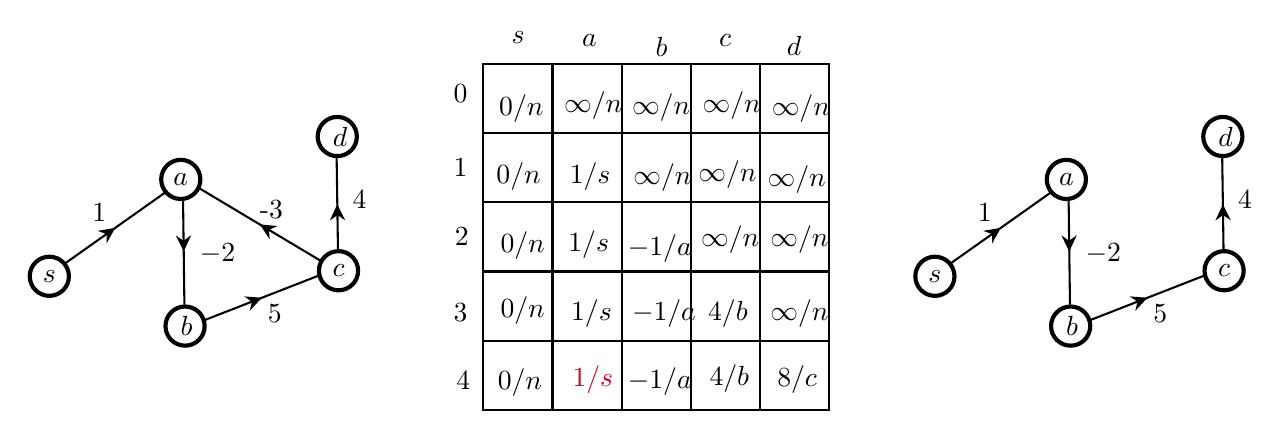
\begin{tikzpicture}[x=0.5pt,y=0.5pt,yscale=-1,xscale=1]
%uncomment if require: \path (0,334); %set diagram left start at 0, and has height of 334

%Shape: Grid [id:dp11668880045661734] 
\draw  [draw opacity=0] (352,45) -- (602,45) -- (602,295) -- (352,295) -- cycle ; \draw   (402,45) -- (402,295)(452,45) -- (452,295)(502,45) -- (502,295)(552,45) -- (552,295) ; \draw   (352,95) -- (602,95)(352,145) -- (602,145)(352,195) -- (602,195)(352,245) -- (602,245) ; \draw   (352,45) -- (602,45) -- (602,295) -- (352,295) -- cycle ;
%Straight Lines [id:da34498379019209924] 
\draw [color={rgb, 255:red, 0; green, 0; blue, 0 }  ,draw opacity=1 ][line width=0.75]    (50,189) -- (122,138) ;
\draw [shift={(86,163.5)}, rotate = 504.69] [fill={rgb, 255:red, 0; green, 0; blue, 0 }  ,fill opacity=1 ][line width=0.08]  [draw opacity=0] (11.61,-5.58) -- (0,0) -- (11.61,5.58) -- (7.71,0) -- cycle    ;
%Straight Lines [id:da15240395104529547] 
\draw [color={rgb, 255:red, 0; green, 0; blue, 0 }  ,draw opacity=1 ][line width=0.75]    (147,135) -- (234,187) ;
\draw [shift={(190.5,161)}, rotate = 30.87] [fill={rgb, 255:red, 0; green, 0; blue, 0 }  ,fill opacity=1 ][line width=0.08]  [draw opacity=0] (11.61,-5.58) -- (0,0) -- (11.61,5.58) -- (7.71,0) -- cycle    ;
%Straight Lines [id:da35482909520855144] 
\draw [color={rgb, 255:red, 0; green, 0; blue, 0 }  ,draw opacity=1 ][line width=0.75]    (233,198) -- (151,230) ;
\draw [shift={(192,214)}, rotate = 158.68] [fill={rgb, 255:red, 0; green, 0; blue, 0 }  ,fill opacity=1 ][line width=0.08]  [draw opacity=0] (11.61,-5.58) -- (0,0) -- (11.61,5.58) -- (7.71,0) -- cycle    ;
%Straight Lines [id:da9934926023449607] 
\draw [color={rgb, 255:red, 0; green, 0; blue, 0 }  ,draw opacity=1 ][line width=0.75]    (135,142) -- (136,219) ;
\draw [shift={(135.5,180.5)}, rotate = 269.26] [fill={rgb, 255:red, 0; green, 0; blue, 0 }  ,fill opacity=1 ][line width=0.08]  [draw opacity=0] (11.61,-5.58) -- (0,0) -- (11.61,5.58) -- (7.71,0) -- cycle    ;
%Straight Lines [id:da7563500509285274] 
\draw [color={rgb, 255:red, 0; green, 0; blue, 0 }  ,draw opacity=1 ][line width=0.75]    (246,112) -- (247,181) ;
\draw [shift={(246.5,146.5)}, rotate = 89.17] [fill={rgb, 255:red, 0; green, 0; blue, 0 }  ,fill opacity=1 ][line width=0.08]  [draw opacity=0] (11.61,-5.58) -- (0,0) -- (11.61,5.58) -- (7.71,0) -- cycle    ;
%Straight Lines [id:da1926158580753592] 
\draw [color={rgb, 255:red, 0; green, 0; blue, 0 }  ,draw opacity=1 ][line width=0.75]    (690,189) -- (762,138) ;
\draw [shift={(726,163.5)}, rotate = 504.69] [fill={rgb, 255:red, 0; green, 0; blue, 0 }  ,fill opacity=1 ][line width=0.08]  [draw opacity=0] (11.61,-5.58) -- (0,0) -- (11.61,5.58) -- (7.71,0) -- cycle    ;
%Straight Lines [id:da5417396008779365] 
\draw [color={rgb, 255:red, 0; green, 0; blue, 0 }  ,draw opacity=1 ][line width=0.75]    (873,198) -- (791,230) ;
\draw [shift={(832,214)}, rotate = 158.68] [fill={rgb, 255:red, 0; green, 0; blue, 0 }  ,fill opacity=1 ][line width=0.08]  [draw opacity=0] (11.61,-5.58) -- (0,0) -- (11.61,5.58) -- (7.71,0) -- cycle    ;
%Straight Lines [id:da8796336265405228] 
\draw [color={rgb, 255:red, 0; green, 0; blue, 0 }  ,draw opacity=1 ][line width=0.75]    (775,142) -- (776,219) ;
\draw [shift={(775.5,180.5)}, rotate = 269.26] [fill={rgb, 255:red, 0; green, 0; blue, 0 }  ,fill opacity=1 ][line width=0.08]  [draw opacity=0] (11.61,-5.58) -- (0,0) -- (11.61,5.58) -- (7.71,0) -- cycle    ;
%Straight Lines [id:da08409930095041618] 
\draw [color={rgb, 255:red, 0; green, 0; blue, 0 }  ,draw opacity=1 ][line width=0.75]    (886,112) -- (887,181) ;
\draw [shift={(886.5,146.5)}, rotate = 89.17] [fill={rgb, 255:red, 0; green, 0; blue, 0 }  ,fill opacity=1 ][line width=0.08]  [draw opacity=0] (11.61,-5.58) -- (0,0) -- (11.61,5.58) -- (7.71,0) -- cycle    ;

% Text Node
\draw (361.24,65.06) node [anchor=north west][inner sep=0.75pt]   [align=left] {$\displaystyle 0/n$};
% Text Node
\draw (328.24,111.56) node [anchor=north west][inner sep=0.75pt]   [align=left] {$\displaystyle 1$};
% Text Node
\draw (329.24,161.06) node [anchor=north west][inner sep=0.75pt]   [align=left] {$\displaystyle 2$};
% Text Node
\draw (370.24,19.56) node [anchor=north west][inner sep=0.75pt]   [align=left] {$\displaystyle s$};
% Text Node
\draw (421.24,21.56) node [anchor=north west][inner sep=0.75pt]   [align=left] {$\displaystyle a$};
% Text Node
\draw (474.24,23.56) node [anchor=north west][inner sep=0.75pt]   [align=left] {$\displaystyle b$};
% Text Node
\draw (520.24,21.56) node [anchor=north west][inner sep=0.75pt]   [align=left] {$\displaystyle c$};
% Text Node
\draw (408.24,63.06) node [anchor=north west][inner sep=0.75pt]   [align=left] {$\displaystyle \infty /n$};
% Text Node
\draw (328.24,58.06) node [anchor=north west][inner sep=0.75pt]   [align=left] {$\displaystyle 0$};
% Text Node
\draw (328.24,216.06) node [anchor=north west][inner sep=0.75pt]   [align=left] {$\displaystyle 3$};
% Text Node
\draw (188.24,141.53) node [anchor=north west][inner sep=0.75pt]   [align=left] {\mbox{-}$\displaystyle 3$};
% Text Node
\draw  [line width=1.5]   (38.38, 198.47) circle [x radius= 14.15, y radius= 14.15]   ;
\draw (38.38,198.47) node   [align=left] {$\displaystyle s$};
% Text Node
\draw  [line width=1.5]   (133.38, 128.47) circle [x radius= 14.15, y radius= 14.15]   ;
\draw (133.38,128.47) node   [align=left] {$\displaystyle a$};
% Text Node
\draw  [line width=1.5]   (136.48, 234.47) circle [x radius= 14.15, y radius= 14.15]   ;
\draw (130.98,234.47) node [anchor=west] [inner sep=0.75pt]   [align=left] {$\displaystyle b$};
% Text Node
\draw  [line width=1.5]   (247.38, 194.47) circle [x radius= 14.15, y radius= 14.15]   ;
\draw (247.38,194.47) node   [align=left] {$\displaystyle c$};
% Text Node
\draw (67.24,143.53) node [anchor=north west][inner sep=0.75pt]   [align=left] {$\displaystyle 1$};
% Text Node
\draw (194,217) node [anchor=north west][inner sep=0.75pt]   [align=left] {$\displaystyle 5$};
% Text Node
\draw (145,172.47) node [anchor=north west][inner sep=0.75pt]   [align=left] {$\displaystyle -2$};
% Text Node
\draw (457.24,64.06) node [anchor=north west][inner sep=0.75pt]   [align=left] {$\displaystyle \infty /n$};
% Text Node
\draw (508.24,63.06) node [anchor=north west][inner sep=0.75pt]   [align=left] {$\displaystyle \infty /n$};
% Text Node
\draw (505.24,113.06) node [anchor=north west][inner sep=0.75pt]   [align=left] {$\displaystyle \infty /n$};
% Text Node
\draw (359.24,114.06) node [anchor=north west][inner sep=0.75pt]   [align=left] {$\displaystyle 0/n$};
% Text Node
\draw (362.24,164.06) node [anchor=north west][inner sep=0.75pt]   [align=left] {$\displaystyle 0/n$};
% Text Node
\draw (362.24,211.06) node [anchor=north west][inner sep=0.75pt]   [align=left] {$\displaystyle 0/n$};
% Text Node
\draw (412.24,114.06) node [anchor=north west][inner sep=0.75pt]   [align=left] {$\displaystyle 1/s$};
% Text Node
\draw (458.24,115.06) node [anchor=north west][inner sep=0.75pt]   [align=left] {$\displaystyle \infty /n$};
% Text Node
\draw (507.24,160.06) node [anchor=north west][inner sep=0.75pt]   [align=left] {$\displaystyle \infty /n$};
% Text Node
\draw (411.24,163.06) node [anchor=north west][inner sep=0.75pt]   [align=left] {$\displaystyle 1/s$};
% Text Node
\draw (454.24,166.06) node [anchor=north west][inner sep=0.75pt]   [align=left] {$\displaystyle -1/a$};
% Text Node
\draw (330.24,265.06) node [anchor=north west][inner sep=0.75pt]   [align=left] {$\displaystyle 4$};
% Text Node
\draw (569.24,22.56) node [anchor=north west][inner sep=0.75pt]   [align=left] {$\displaystyle d$};
% Text Node
\draw  [line width=1.5]   (246.48, 97.47) circle [x radius= 14.15, y radius= 14.15]   ;
\draw (240.98,97.47) node [anchor=west] [inner sep=0.75pt]   [align=left] {$\displaystyle d$};
% Text Node
\draw (255.24,134.53) node [anchor=north west][inner sep=0.75pt]   [align=left] {$\displaystyle 4$};
% Text Node
\draw (558.24,65.06) node [anchor=north west][inner sep=0.75pt]   [align=left] {$\displaystyle \infty /n$};
% Text Node
\draw (555.24,116.06) node [anchor=north west][inner sep=0.75pt]   [align=left] {$\displaystyle \infty /n$};
% Text Node
\draw (557.24,160.06) node [anchor=north west][inner sep=0.75pt]   [align=left] {$\displaystyle \infty /n$};
% Text Node
\draw (557.24,213.06) node [anchor=north west][inner sep=0.75pt]   [align=left] {$\displaystyle \infty /n$};
% Text Node
\draw (360.24,263.06) node [anchor=north west][inner sep=0.75pt]   [align=left] {$\displaystyle 0/n$};
% Text Node
\draw (413.24,213.06) node [anchor=north west][inner sep=0.75pt]   [align=left] {$\displaystyle 1/s$};
% Text Node
\draw (457.24,213.06) node [anchor=north west][inner sep=0.75pt]   [align=left] {$\displaystyle -1/a$};
% Text Node
\draw (454.24,262.06) node [anchor=north west][inner sep=0.75pt]   [align=left] {$\displaystyle -1/a$};
% Text Node
\draw (512.24,213.06) node [anchor=north west][inner sep=0.75pt]   [align=left] {$\displaystyle 4/b$};
% Text Node
\draw (513.24,260.06) node [anchor=north west][inner sep=0.75pt]   [align=left] {$\displaystyle 4/b$};
% Text Node
\draw (562.24,261.06) node [anchor=north west][inner sep=0.75pt]   [align=left] {$\displaystyle 8/c$};
% Text Node
\draw (414.24,261.06) node [anchor=north west][inner sep=0.75pt]  [color={rgb, 255:red, 208; green, 2; blue, 27 }  ,opacity=1 ] [align=left] {$\displaystyle 1/s$};
% Text Node
\draw  [line width=1.5]   (678.38, 198.47) circle [x radius= 14.15, y radius= 14.15]   ;
\draw (678.38,198.47) node   [align=left] {$\displaystyle s$};
% Text Node
\draw  [line width=1.5]   (773.38, 128.47) circle [x radius= 14.15, y radius= 14.15]   ;
\draw (773.38,128.47) node   [align=left] {$\displaystyle a$};
% Text Node
\draw  [line width=1.5]   (776.48, 234.47) circle [x radius= 14.15, y radius= 14.15]   ;
\draw (770.98,234.47) node [anchor=west] [inner sep=0.75pt]   [align=left] {$\displaystyle b$};
% Text Node
\draw  [line width=1.5]   (887.38, 194.47) circle [x radius= 14.15, y radius= 14.15]   ;
\draw (887.38,194.47) node   [align=left] {$\displaystyle c$};
% Text Node
\draw (707.24,143.53) node [anchor=north west][inner sep=0.75pt]   [align=left] {$\displaystyle 1$};
% Text Node
\draw (834,217) node [anchor=north west][inner sep=0.75pt]   [align=left] {$\displaystyle 5$};
% Text Node
\draw (785,172.47) node [anchor=north west][inner sep=0.75pt]   [align=left] {$\displaystyle -2$};
% Text Node
\draw  [line width=1.5]   (886.48, 97.47) circle [x radius= 14.15, y radius= 14.15]   ;
\draw (880.98,97.47) node [anchor=west] [inner sep=0.75pt]   [align=left] {$\displaystyle d$};
% Text Node
\draw (895.24,134.53) node [anchor=north west][inner sep=0.75pt]   [align=left] {$\displaystyle 4$};


\end{tikzpicture}

}
%%\caption{Using ``$>$'' to break tie. In this case the shortest-path graph constructed from $prev$ array is guaranteed to be a shortest path tree.
%%	The $prev$ is next to $dist$ separated with $/$ in each entry.}
%%\label{fig:cycle1}
%%\end{figure}
%%
%%\begin{figure}[t]
%%\centering{

\tikzset{every picture/.style={line width=0.75pt}} %set default line width to 0.75pt        

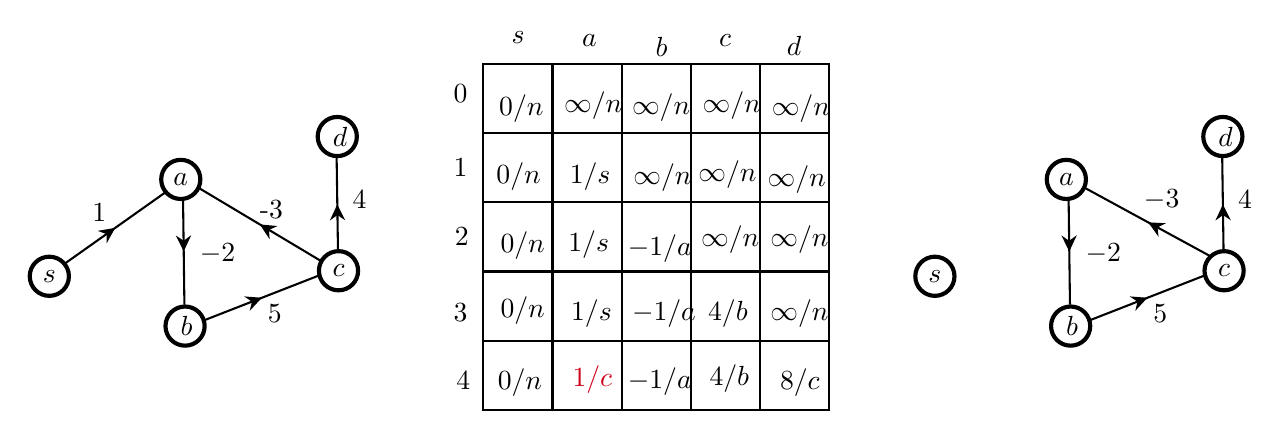
\begin{tikzpicture}[x=0.5pt,y=0.5pt,yscale=-1,xscale=1]
%uncomment if require: \path (0,334); %set diagram left start at 0, and has height of 334

%Shape: Grid [id:dp11668880045661734] 
\draw  [draw opacity=0] (352,45) -- (602,45) -- (602,295) -- (352,295) -- cycle ; \draw   (402,45) -- (402,295)(452,45) -- (452,295)(502,45) -- (502,295)(552,45) -- (552,295) ; \draw   (352,95) -- (602,95)(352,145) -- (602,145)(352,195) -- (602,195)(352,245) -- (602,245) ; \draw   (352,45) -- (602,45) -- (602,295) -- (352,295) -- cycle ;
%Straight Lines [id:da34498379019209924] 
\draw [color={rgb, 255:red, 0; green, 0; blue, 0 }  ,draw opacity=1 ][line width=0.75]    (50,189) -- (122,138) ;
\draw [shift={(86,163.5)}, rotate = 504.69] [fill={rgb, 255:red, 0; green, 0; blue, 0 }  ,fill opacity=1 ][line width=0.08]  [draw opacity=0] (11.61,-5.58) -- (0,0) -- (11.61,5.58) -- (7.71,0) -- cycle    ;
%Straight Lines [id:da15240395104529547] 
\draw [color={rgb, 255:red, 0; green, 0; blue, 0 }  ,draw opacity=1 ][line width=0.75]    (147,135) -- (234,187) ;
\draw [shift={(190.5,161)}, rotate = 30.87] [fill={rgb, 255:red, 0; green, 0; blue, 0 }  ,fill opacity=1 ][line width=0.08]  [draw opacity=0] (11.61,-5.58) -- (0,0) -- (11.61,5.58) -- (7.71,0) -- cycle    ;
%Straight Lines [id:da35482909520855144] 
\draw [color={rgb, 255:red, 0; green, 0; blue, 0 }  ,draw opacity=1 ][line width=0.75]    (233,198) -- (151,230) ;
\draw [shift={(192,214)}, rotate = 158.68] [fill={rgb, 255:red, 0; green, 0; blue, 0 }  ,fill opacity=1 ][line width=0.08]  [draw opacity=0] (11.61,-5.58) -- (0,0) -- (11.61,5.58) -- (7.71,0) -- cycle    ;
%Straight Lines [id:da9934926023449607] 
\draw [color={rgb, 255:red, 0; green, 0; blue, 0 }  ,draw opacity=1 ][line width=0.75]    (135,142) -- (136,219) ;
\draw [shift={(135.5,180.5)}, rotate = 269.26] [fill={rgb, 255:red, 0; green, 0; blue, 0 }  ,fill opacity=1 ][line width=0.08]  [draw opacity=0] (11.61,-5.58) -- (0,0) -- (11.61,5.58) -- (7.71,0) -- cycle    ;
%Straight Lines [id:da7563500509285274] 
\draw [color={rgb, 255:red, 0; green, 0; blue, 0 }  ,draw opacity=1 ][line width=0.75]    (246,112) -- (247,181) ;
\draw [shift={(246.5,146.5)}, rotate = 89.17] [fill={rgb, 255:red, 0; green, 0; blue, 0 }  ,fill opacity=1 ][line width=0.08]  [draw opacity=0] (11.61,-5.58) -- (0,0) -- (11.61,5.58) -- (7.71,0) -- cycle    ;
%Straight Lines [id:da1926158580753592] 
\draw [color={rgb, 255:red, 0; green, 0; blue, 0 }  ,draw opacity=1 ][line width=0.75]    (787.5,135) -- (877.5,184) ;
\draw [shift={(832.5,159.5)}, rotate = 28.57] [fill={rgb, 255:red, 0; green, 0; blue, 0 }  ,fill opacity=1 ][line width=0.08]  [draw opacity=0] (11.61,-5.58) -- (0,0) -- (11.61,5.58) -- (7.71,0) -- cycle    ;
%Straight Lines [id:da5417396008779365] 
\draw [color={rgb, 255:red, 0; green, 0; blue, 0 }  ,draw opacity=1 ][line width=0.75]    (873,198) -- (791,230) ;
\draw [shift={(832,214)}, rotate = 158.68] [fill={rgb, 255:red, 0; green, 0; blue, 0 }  ,fill opacity=1 ][line width=0.08]  [draw opacity=0] (11.61,-5.58) -- (0,0) -- (11.61,5.58) -- (7.71,0) -- cycle    ;
%Straight Lines [id:da8796336265405228] 
\draw [color={rgb, 255:red, 0; green, 0; blue, 0 }  ,draw opacity=1 ][line width=0.75]    (775,142) -- (776,219) ;
\draw [shift={(775.5,180.5)}, rotate = 269.26] [fill={rgb, 255:red, 0; green, 0; blue, 0 }  ,fill opacity=1 ][line width=0.08]  [draw opacity=0] (11.61,-5.58) -- (0,0) -- (11.61,5.58) -- (7.71,0) -- cycle    ;
%Straight Lines [id:da08409930095041618] 
\draw [color={rgb, 255:red, 0; green, 0; blue, 0 }  ,draw opacity=1 ][line width=0.75]    (886,112) -- (887,181) ;
\draw [shift={(886.5,146.5)}, rotate = 89.17] [fill={rgb, 255:red, 0; green, 0; blue, 0 }  ,fill opacity=1 ][line width=0.08]  [draw opacity=0] (11.61,-5.58) -- (0,0) -- (11.61,5.58) -- (7.71,0) -- cycle    ;

% Text Node
\draw (361.24,65.06) node [anchor=north west][inner sep=0.75pt]   [align=left] {$\displaystyle 0/n$};
% Text Node
\draw (328.24,111.56) node [anchor=north west][inner sep=0.75pt]   [align=left] {$\displaystyle 1$};
% Text Node
\draw (329.24,161.06) node [anchor=north west][inner sep=0.75pt]   [align=left] {$\displaystyle 2$};
% Text Node
\draw (370.24,19.56) node [anchor=north west][inner sep=0.75pt]   [align=left] {$\displaystyle s$};
% Text Node
\draw (421.24,21.56) node [anchor=north west][inner sep=0.75pt]   [align=left] {$\displaystyle a$};
% Text Node
\draw (474.24,23.56) node [anchor=north west][inner sep=0.75pt]   [align=left] {$\displaystyle b$};
% Text Node
\draw (520.24,21.56) node [anchor=north west][inner sep=0.75pt]   [align=left] {$\displaystyle c$};
% Text Node
\draw (408.24,63.06) node [anchor=north west][inner sep=0.75pt]   [align=left] {$\displaystyle \infty /n$};
% Text Node
\draw (328.24,58.06) node [anchor=north west][inner sep=0.75pt]   [align=left] {$\displaystyle 0$};
% Text Node
\draw (328.24,216.06) node [anchor=north west][inner sep=0.75pt]   [align=left] {$\displaystyle 3$};
% Text Node
\draw (188.24,141.53) node [anchor=north west][inner sep=0.75pt]   [align=left] {\mbox{-}$\displaystyle 3$};
% Text Node
\draw  [line width=1.5]   (38.38, 198.47) circle [x radius= 14.15, y radius= 14.15]   ;
\draw (38.38,198.47) node   [align=left] {$\displaystyle s$};
% Text Node
\draw  [line width=1.5]   (133.38, 128.47) circle [x radius= 14.15, y radius= 14.15]   ;
\draw (133.38,128.47) node   [align=left] {$\displaystyle a$};
% Text Node
\draw  [line width=1.5]   (136.48, 234.47) circle [x radius= 14.15, y radius= 14.15]   ;
\draw (130.98,234.47) node [anchor=west] [inner sep=0.75pt]   [align=left] {$\displaystyle b$};
% Text Node
\draw  [line width=1.5]   (247.38, 194.47) circle [x radius= 14.15, y radius= 14.15]   ;
\draw (247.38,194.47) node   [align=left] {$\displaystyle c$};
% Text Node
\draw (67.24,143.53) node [anchor=north west][inner sep=0.75pt]   [align=left] {$\displaystyle 1$};
% Text Node
\draw (194,217) node [anchor=north west][inner sep=0.75pt]   [align=left] {$\displaystyle 5$};
% Text Node
\draw (145,172.47) node [anchor=north west][inner sep=0.75pt]   [align=left] {$\displaystyle -2$};
% Text Node
\draw (457.24,64.06) node [anchor=north west][inner sep=0.75pt]   [align=left] {$\displaystyle \infty /n$};
% Text Node
\draw (508.24,63.06) node [anchor=north west][inner sep=0.75pt]   [align=left] {$\displaystyle \infty /n$};
% Text Node
\draw (505.24,113.06) node [anchor=north west][inner sep=0.75pt]   [align=left] {$\displaystyle \infty /n$};
% Text Node
\draw (359.24,114.06) node [anchor=north west][inner sep=0.75pt]   [align=left] {$\displaystyle 0/n$};
% Text Node
\draw (362.24,164.06) node [anchor=north west][inner sep=0.75pt]   [align=left] {$\displaystyle 0/n$};
% Text Node
\draw (362.24,211.06) node [anchor=north west][inner sep=0.75pt]   [align=left] {$\displaystyle 0/n$};
% Text Node
\draw (412.24,114.06) node [anchor=north west][inner sep=0.75pt]   [align=left] {$\displaystyle 1/s$};
% Text Node
\draw (458.24,115.06) node [anchor=north west][inner sep=0.75pt]   [align=left] {$\displaystyle \infty /n$};
% Text Node
\draw (507.24,160.06) node [anchor=north west][inner sep=0.75pt]   [align=left] {$\displaystyle \infty /n$};
% Text Node
\draw (411.24,163.06) node [anchor=north west][inner sep=0.75pt]   [align=left] {$\displaystyle 1/s$};
% Text Node
\draw (454.24,166.06) node [anchor=north west][inner sep=0.75pt]   [align=left] {$\displaystyle -1/a$};
% Text Node
\draw (330.24,265.06) node [anchor=north west][inner sep=0.75pt]   [align=left] {$\displaystyle 4$};
% Text Node
\draw (569.24,22.56) node [anchor=north west][inner sep=0.75pt]   [align=left] {$\displaystyle d$};
% Text Node
\draw  [line width=1.5]   (246.48, 97.47) circle [x radius= 14.15, y radius= 14.15]   ;
\draw (240.98,97.47) node [anchor=west] [inner sep=0.75pt]   [align=left] {$\displaystyle d$};
% Text Node
\draw (255.24,134.53) node [anchor=north west][inner sep=0.75pt]   [align=left] {$\displaystyle 4$};
% Text Node
\draw (558.24,65.06) node [anchor=north west][inner sep=0.75pt]   [align=left] {$\displaystyle \infty /n$};
% Text Node
\draw (555.24,116.06) node [anchor=north west][inner sep=0.75pt]   [align=left] {$\displaystyle \infty /n$};
% Text Node
\draw (557.24,160.06) node [anchor=north west][inner sep=0.75pt]   [align=left] {$\displaystyle \infty /n$};
% Text Node
\draw (557.24,213.06) node [anchor=north west][inner sep=0.75pt]   [align=left] {$\displaystyle \infty /n$};
% Text Node
\draw (360.24,263.06) node [anchor=north west][inner sep=0.75pt]   [align=left] {$\displaystyle 0/n$};
% Text Node
\draw (413.24,213.06) node [anchor=north west][inner sep=0.75pt]   [align=left] {$\displaystyle 1/s$};
% Text Node
\draw (457.24,213.06) node [anchor=north west][inner sep=0.75pt]   [align=left] {$\displaystyle -1/a$};
% Text Node
\draw (454.24,262.06) node [anchor=north west][inner sep=0.75pt]   [align=left] {$\displaystyle -1/a$};
% Text Node
\draw (512.24,213.06) node [anchor=north west][inner sep=0.75pt]   [align=left] {$\displaystyle 4/b$};
% Text Node
\draw (513.24,260.06) node [anchor=north west][inner sep=0.75pt]   [align=left] {$\displaystyle 4/b$};
% Text Node
\draw (564.24,263.06) node [anchor=north west][inner sep=0.75pt]   [align=left] {$\displaystyle 8/c$};
% Text Node
\draw (414.24,261.06) node [anchor=north west][inner sep=0.75pt]  [color={rgb, 255:red, 208; green, 2; blue, 27 }  ,opacity=1 ] [align=left] {$\displaystyle 1/c$};
% Text Node
\draw  [line width=1.5]   (678.38, 198.47) circle [x radius= 14.15, y radius= 14.15]   ;
\draw (678.38,198.47) node   [align=left] {$\displaystyle s$};
% Text Node
\draw  [line width=1.5]   (773.38, 128.47) circle [x radius= 14.15, y radius= 14.15]   ;
\draw (773.38,128.47) node   [align=left] {$\displaystyle a$};
% Text Node
\draw  [line width=1.5]   (776.48, 234.47) circle [x radius= 14.15, y radius= 14.15]   ;
\draw (770.98,234.47) node [anchor=west] [inner sep=0.75pt]   [align=left] {$\displaystyle b$};
% Text Node
\draw  [line width=1.5]   (887.38, 194.47) circle [x radius= 14.15, y radius= 14.15]   ;
\draw (887.38,194.47) node   [align=left] {$\displaystyle c$};
% Text Node
\draw (827.24,133.53) node [anchor=north west][inner sep=0.75pt]   [align=left] {$\displaystyle -3$};
% Text Node
\draw (834,217) node [anchor=north west][inner sep=0.75pt]   [align=left] {$\displaystyle 5$};
% Text Node
\draw (785,172.47) node [anchor=north west][inner sep=0.75pt]   [align=left] {$\displaystyle -2$};
% Text Node
\draw  [line width=1.5]   (886.48, 97.47) circle [x radius= 14.15, y radius= 14.15]   ;
\draw (880.98,97.47) node [anchor=west] [inner sep=0.75pt]   [align=left] {$\displaystyle d$};
% Text Node
\draw (895.24,134.53) node [anchor=north west][inner sep=0.75pt]   [align=left] {$\displaystyle 4$};


\end{tikzpicture}

}
%%\caption{Using ``$\ge$'' to break tie. In this case the shortest-path graph constructed from $prev$ array may not be a shortest path tree.
%%	The $prev$ is next to $dist$ separated with $/$ in each entry.}
%%\label{fig:cycle2}
%%\end{figure}
%%
%%
%%
%%
